\documentclass[tikz]{standalone}
\usepackage{bm}
\usetikzlibrary{patterns}
\newcommand{\vect}{\bm}
\newcommand{\del}{\boldsymbol{\nabla}}

\newcommand{\trans}[1]{{#1^\star}}
\newcommand{\surface}{h}
\newcommand{\shellcmd}[1]{\texttt{#1}}
\newcommand{\diffusioncoeff}{\mathcal{D}}
\newcommand{\exner}{\Pi}

\begin{document}
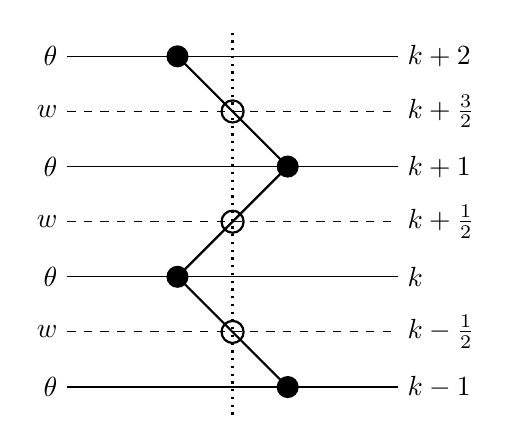
\begin{tikzpicture}[
  scale=0.7,
  cpnt/.style={fill=black}
]
\draw (0,0) -- (6,0) node [at start, anchor=east] {$\theta$} node [at end, anchor=west] {$k-1$};
\draw [dashed] (0,1) -- (6,1) node [at start, anchor=east] {$w$} node [at end, anchor=west] {$k-\frac{1}{2}$};
\draw (0,2) -- (6,2) node [at start, anchor=east] {$\theta$} node [at end, anchor=west] {$k$};
\draw [dashed] (0,3) -- (6,3) node [at start, anchor=east] {$w$} node [at end, anchor=west] {$k+\frac{1}{2}$};
\draw (0,4) -- (6,4) node [at start, anchor=east] {$\theta$} node [at end, anchor=west] {$k+1$};
\draw [dashed] (0,5) -- (6,5) node [at start, anchor=east] {$w$} node [at end, anchor=west] {$k+\frac{3}{2}$};
\draw (0,6) -- (6,6) node [at start, anchor=east] {$\theta$} node [at end, anchor=west] {$k+2$};

\path [cpnt] (4,0) circle [radius=0.2];
\path [cpnt] (2,2) circle [radius=0.2];
\path [cpnt] (4,4) circle [radius=0.2];
\path [cpnt] (2,6) circle [radius=0.2];
\draw [thick] (3,1) circle [radius=0.2];
\draw [thick] (3,3) circle [radius=0.2];
\draw [thick] (3,5) circle [radius=0.2];

\draw [thick] (4,0) -- (2,2) -- (4,4) -- (2,6);
\draw [thick, dotted] (3,-0.5) -- (3,6.5);
\end{tikzpicture}
\end{document}
